    
% \subsubsection{Omnidirectional mode}
% \label{subsec:omnidirectional_mode}

%     As aforementioned, to activate the omnidirectional mode, the standard wheels should be replaced with Mecanum wheels (see Figure \ref{fig:MecanumKin}). Additionally, two other actions are required to operate in this mode, namely (i) enable the "Mecanum mode" using the Nexus app, as described in Subsection \ref{subsec:limo_app} (notice that this mode can only be activated via the Nexus app and cannot be enabled directly through ROS), and (ii) modify the file \texttt{limo\_base.launch} by setting the \texttt{use\_mecanum} argument to \texttt{true} when in omnidirectional mode and to \texttt{false} in other modes.
    
%     In omnidirectional mode, longitudinal and lateral movements are independent of the vehicle's orientation. To distinguish the states in this mode, we use the subscript `o' to refer to the states measured relative to the center of mass of the omnidirectional robot. Unlike the differential mode, the position offset $a$ is not used in omnidirectional mode. Still, the state vector is expanded to include the orientation $\psi$, becoming $\bs x_o = \begin{bmatrix} x & y & \psi \end{bmatrix}^T$.
    
%     \begin{figure}[!b]
%         \centering
%         \includegraphics[viewport=20 90 250 280, clip, width=0.8\linewidth]{images/CinematicaMecanum_2.jpg}
%         \caption{Kinematics of the omnidirectional LIMO robot.}
%         \label{fig:MecanumKin}
%     \end{figure}
    
%     In this operation mode, the control input consists of the longitudinal and side linear velocities, respectively $\dot{x}^b$ and $\dot{y}^b$, and of the angular velocity $\omega$. Therefore, the kinematic model for the omnidirectional mode, obtained from Figure~\ref{fig:MecanumKin}, is $\dot{\bs x}_{o} = \bs H_o \bs u_o$ \cite{Sarcinelli-Filho2023_2}, or
%     \begin{equation}
%         \bs{x}_{o}=\begin{bmatrix} \dot{x} \\ \dot{y} \\  \dot{\psi}  \end{bmatrix} = \begin{bmatrix} c_\psi & -s_\psi & 0 \\ s_\psi & c_\psi & 0 \\ 0 & 0 & 1 \end{bmatrix}  \begin{bmatrix} \dot{x}^b \\ \dot{y}^b \\ \omega \end{bmatrix}.
%     \end{equation}
%     \noindent The kinematic controller is obtained using the inverse kinematics once more, such that $\bs u_o = \bs H_o^{-1} \dot{\bs{x}}_{o,ref} $ \cite{Sarcinelli-Filho2023_4}, or
%     \begin{equation}
%         \begin{bmatrix} \dot{x}^b \\ \dot{y}^b \\ \omega \end{bmatrix} = \begin{bmatrix} c_\psi & s_\psi & 0 \\ -s_\psi & c_\psi & 0 \\ 0 & 0 & 1 \end{bmatrix} \begin{bmatrix} \dot{x}_{ref} \\ \dot{y}_{ref} \\  \dot{\psi}_{ref}  \end{bmatrix},
%     \end{equation}
%     \noindent where $\dot{\bs{x}}_{o,ref}$ can be as in \eqref{eq:ff_fb_law}.

\subsubsection{Modo omnidirecional}
    \label{subsec:omnidirectional_mode}
    
    Como mencionado anteriormente, para ativar o modo omnidirecional, as rodas padrão devem ser substituídas por rodas Mecanum (veja a Figura \ref{fig:MecanumKin}). Além disso, duas outras ações são necessárias para operar neste modo, a saber: (i) habilitar o "modo Mecanum" usando o aplicativo Nexus (observe que este modo só pode ser ativado via aplicativo Nexus e não pode ser habilitado diretamente através do ROS), e (ii) modificar o arquivo \texttt{limo\_base.launch} configurando o argumento \texttt{use\_mecanum} como \texttt{true} quando no modo omnidirecional e \texttt{false} em outros modos.
    
    No modo omnidirecional, os movimentos longitudinais e laterais são independentes da orientação do veículo. Para distinguir os estados neste modo, usamos o subscrito 'o' para nos referirmos aos estados medidos em relação ao centro de massa do robô omnidirecional. Ao contrário do modo diferencial, o deslocamento de posição $a$ não é utilizado no modo omnidirecional. Ainda assim, o vetor de estado é expandido para incluir a orientação $\psi$, tornando-se $\bs x_o = \begin{bmatrix} x & y & \psi \end{bmatrix}^T$.
    
    \begin{figure}[htb]
        \centering
        \caption{Cinemática do robô LIMO em modo omnidirecional.}
        \includegraphics[viewport=20 90 250 280, clip, width=0.3\linewidth]{CinematicaMecanum_2.jpg}
        
        \label{fig:MecanumKin}
    \end{figure}
    
    Neste modo de operação, a entrada de controle consiste nas velocidades lineares longitudinais e laterais, respectivamente $\dot{x}^b$ e $\dot{y}^b$, e da velocidade angular $\omega$. Portanto, o modelo cinemático para o modo omnidirecional, obtido a partir da Figura~\ref{fig:MecanumKin}, é $\dot{\bs x}_{o} = \bs H_o \bs u_o$ \cite{Sarcinelli-Filho2023_2}, ou
    \begin{equation}
        \bs{x}_{o}=\begin{bmatrix} \dot{x} \\ \dot{y} \\  \dot{\psi}  \end{bmatrix} = \begin{bmatrix} c_\psi & -s_\psi & 0 \\ s_\psi & c_\psi & 0 \\ 0 & 0 & 1 \end{bmatrix}  \begin{bmatrix} \dot{x}^b \\ \dot{y}^b \\ \omega \end{bmatrix}.
    \end{equation}
    \noindent O controlador cinemático é obtido utilizando a cinemática inversa mais uma vez, de modo que $\bs u_o = \bs H_o^{-1} \dot{\bs{x}}_{o,ref} $ \cite{Sarcinelli-Filho2023_4}, ou
    \begin{equation}
        \begin{bmatrix} \dot{x}^b \\ \dot{y}^b \\ \omega \end{bmatrix} = \begin{bmatrix} c_\psi & s_\psi & 0 \\ -s_\psi & c_\psi & 0 \\ 0 & 0 & 1 \end{bmatrix} \begin{bmatrix} \dot{x}_{ref} \\ \dot{y}_{ref} \\  \dot{\psi}_{ref}  \end{bmatrix},
    \end{equation}
    \noindent onde $\dot{\bs{x}}_{o,ref}$ pode ser conforme na \eqref{eq:ff_fb_law}.
    
    